\begin{figure}[h]
\centering
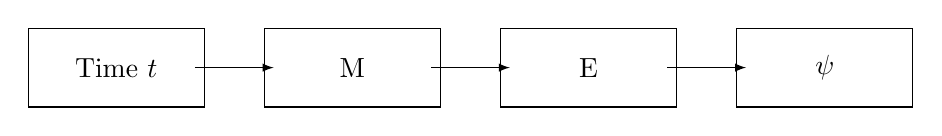
\begin{tikzpicture}
% draw rectangle node
	\node[draw,
		minimum width=2cm,
		minimum height=1cm,
		align=center,
		text width=2cm] at (0,0) {Time $t$};
	\node[draw,
		minimum width=2cm,
		minimum height=1cm,
		align=center,
		text width=2cm] at (3,0) {M};
	\node[draw,
		minimum width=2cm,
		minimum height=1cm,
		align=center,
		text width=2cm] at (6,0) {E};
	\node[draw,
		minimum width=2cm,
		minimum height=1cm,
		align=center,
		text width=2cm] at (9,0) {$\psi$};

    \draw[-latex] (1,0) -- (2,0);
    \draw[-latex] (4,0) -- (5,0);
    \draw[-latex] (7,0) -- (8,0);
\end{tikzpicture}
\caption{Time to State Transition}
\label{fig:2}
\end{figure}

